%%%%%%%%%%%%%%%%%%%%%%%%%%%%%%%%%%%%%%%%%
% Programming/Coding Assignment
% LaTeX Template
%
% This template has been downloaded from:
% http://www.latextemplates.com
%
% Original author:
% Ted Pavlic (http://www.tedpavlic.com)
%
% Note:
% The \lipsum[#] commands throughout this template generate dummy text
% to fill the template out. These commands should all be removed when 
% writing assignment content.
%
% This template uses a Perl script as an example snippet of code, most other
% languages are also usable. Configure them in the "CODE INCLUSION 
% CONFIGURATION" section.
%
%%%%%%%%%%%%%%%%%%%%%%%%%%%%%%%%%%%%%%%%%

%----------------------------------------------------------------------------------------
%	PACKAGES AND OTHER DOCUMENT CONFIGURATIONS
%----------------------------------------------------------------------------------------

\documentclass{article}

\usepackage{fancyhdr} % Required for custom headers
\usepackage{lastpage} % Required to determine the last page for the footer
\usepackage{extramarks} % Required for headers and footers
\usepackage[usenames,dvipsnames]{color} % Required for custom colors
\usepackage{graphicx} % Required to insert images
\usepackage{listings} % Required for insertion of code
\usepackage{courier} % Required for the courier font
\usepackage{multirow}
\usepackage{hyperref}
\usepackage{amsmath}
\usepackage{amssymb}


% Margins
\topmargin=-0.45in
\evensidemargin=0in
\oddsidemargin=0in
\textwidth=6.5in
\textheight=9.0in
\headsep=0.25in

\linespread{1.1} % Line spacing

%----------------------------------------------------------------------------------------
%	CODE INCLUSION CONFIGURATION
%----------------------------------------------------------------------------------------

\definecolor{MyDarkGreen}{rgb}{0.0,0.4,0.0} % This is the color used for comments
\lstloadlanguages{c} % Load Perl syntax for listings, for a list of other languages supported see: ftp://ftp.tex.ac.uk/tex-archive/macros/latex/contrib/listings/listings.pdf
\lstset{language=[sharp]c, % Use Perl in this example
        frame=single, % Single frame around code
        basicstyle=\small\ttfamily, % Use small true type font
        keywordstyle=[1]\color{Blue}\bf, % Perl functions bold and blue
        keywordstyle=[2]\color{Purple}, % Perl function arguments purple
        keywordstyle=[3]\color{Blue}\underbar, % Custom functions underlined and blue
        identifierstyle=, % Nothing special about identifiers                                         
        commentstyle=\usefont{T1}{pcr}{m}{sl}\color{MyDarkGreen}\small, % Comments small dark green courier font
        stringstyle=\color{Purple}, % Strings are purple
        showstringspaces=false, % Don't put marks in string spaces
        tabsize=5, % 5 spaces per tab
        %
        % Put standard Perl functions not included in the default language here
        morekeywords={rand},
        %
        % Put Perl function parameters here
        morekeywords=[2]{on, off, interp},
        %
        % Put user defined functions here
        morekeywords=[3]{test},
       	%
        morecomment=[l][\color{Blue}]{...}, % Line continuation (...) like blue comment
        numbers=left, % Line numbers on left
        firstnumber=1, % Line numbers start with line 1
        numberstyle=\tiny\color{Blue}, % Line numbers are blue and small
        stepnumber=5 % Line numbers go in steps of 5
}

\newcommand{\horrule}[1]{\rule{\linewidth}{#1}}

% Creates a new command to include a perl script, the first parameter is the filename of the script (without .pl), the second parameter is the caption
\newcommand{\perlscript}[2]{
\begin{itemize}
\item[]\lstinputlisting[caption=#2,label=#1]{#1.cs}
\end{itemize}
}

\begin{document}

\begin{tabular}{l l}
\multirow{5}{*}{\includegraphics[width=2cm]{../../recursos/logo.png}} & Universidad del Istmo de Guatemala \\
 & Facultad de Ingenieria \\
 & Ing. en Sistemas \\
 & Informatica 1 \\
 & Prof. Ernesto Rodriguez - \href{mailto:erodriguez@unis.edu.gt}{erodriguez@unis.edu.gt} \\
\end{tabular}
\\\\\\

\begin{center}
        \horrule{0.5pt}
        \huge{Proyecto Final: Fractales} \\
        \large{Fecha de entrega: 01 de Noviembre, 2018 - 11:59pm} \\
        \horrule{1pt}
\end{center}

\emph{Instrucciones: Resolver cada uno de los ejercicios siguiendo sus respectivas
instrucciones. El trabajo debe ser entregado a traves de Github, en su repositorio del curso, colocado en una carpeta llamada "Proyecto Final".
Al menos que la pregunta indique diferente, todas las respuestas a preguntas escritas deben presentarse en
un documento formato pdf, el cual haya sido generado mediante Latex. }
\\\\
A continuaci\'on se presenta el proyecto final. El objetivo de este proyecto es familiarizar al
estudiante con la utilizaci\'on de la programaci\'on funcional para crear programas interactivos.
El objetivo es que el estudiante construya un programa que dibuje fractales.
\\\\
Para este proyecto pude utilizar como machote ya sea el codigo de esta carpeta o el proyecto
ubicado en \url{https://ellie-app.com/3tH24kjVKPJa1}. Si utiliza el proyecto del link, por favor
cree su propia copia en vez de modificar el codigo del link directamente para que sus coma\~neros
puedan obtener una copia sin modificaci\'on si lo desean.
\\\\
El proyecto se puede llevar a cabo de forma individual o en pareja. Si se realiza en pareja,
por favor indicar claramente quien es su pareja y asegurarse que exista una copia del proyecto
en el repositorio de ambos. Este proyecto tiene como valor 15 puntos de los 40 que conforman
el examen final. Adicionalmente, existe la oportunidad de 15 puntos extra de los cuales 5
seran para el examen final y 10 para recuperar nota en los parciales anteriores.
\\\\
Aparte de la entrega final, el dia 01 de noviembre, tendra que presentarle el codigo
al profesor durante la clase. El profesor tiene derecho de hacerle preguntas sobre
cualquier parte del codigo a cualquiera de los integrantes del grupo. La nota final
del proyecto es individual (no en pareja) y dependera de la habilidad de cada integrante
en responder las preguntas que el profesor le haga sobre el codigo.
\section*{Iniciaci\'on}
Esta secci\'on solo importa si va utilizar este repositorio como machote. Si utilizara
el codigo ubicado en Ellie, puede ignorar esta secci\'on. Para utilizar este repositorio
como machote, debe seguir los siguientes pasos:
\begin{enumerate}
        \item{Copiar el contenido de esta carpeta a su carpeta llamada ``Proyecto Final''}
        \item{Navegar a la carpeta ``Proyecto Final'' en la terminal}
        \item{Ejecutar $\mathtt{npm\ install}$ en la terminal}
        \item{Ejecutar $\mathtt{npm\ run\ build}$ en la terminal}
        \item{Ejecutar $\mathtt{node\_modules/.bin/elm\ reactor}$ en la terminal}
        \item{Navegar a \url{http://localhost:8000/index.html} en su navegador y verificar
        que el codigo funciona}
\end{enumerate}
\section*{Copo de Nieve de Koch (5pts)}
\begin{center}
        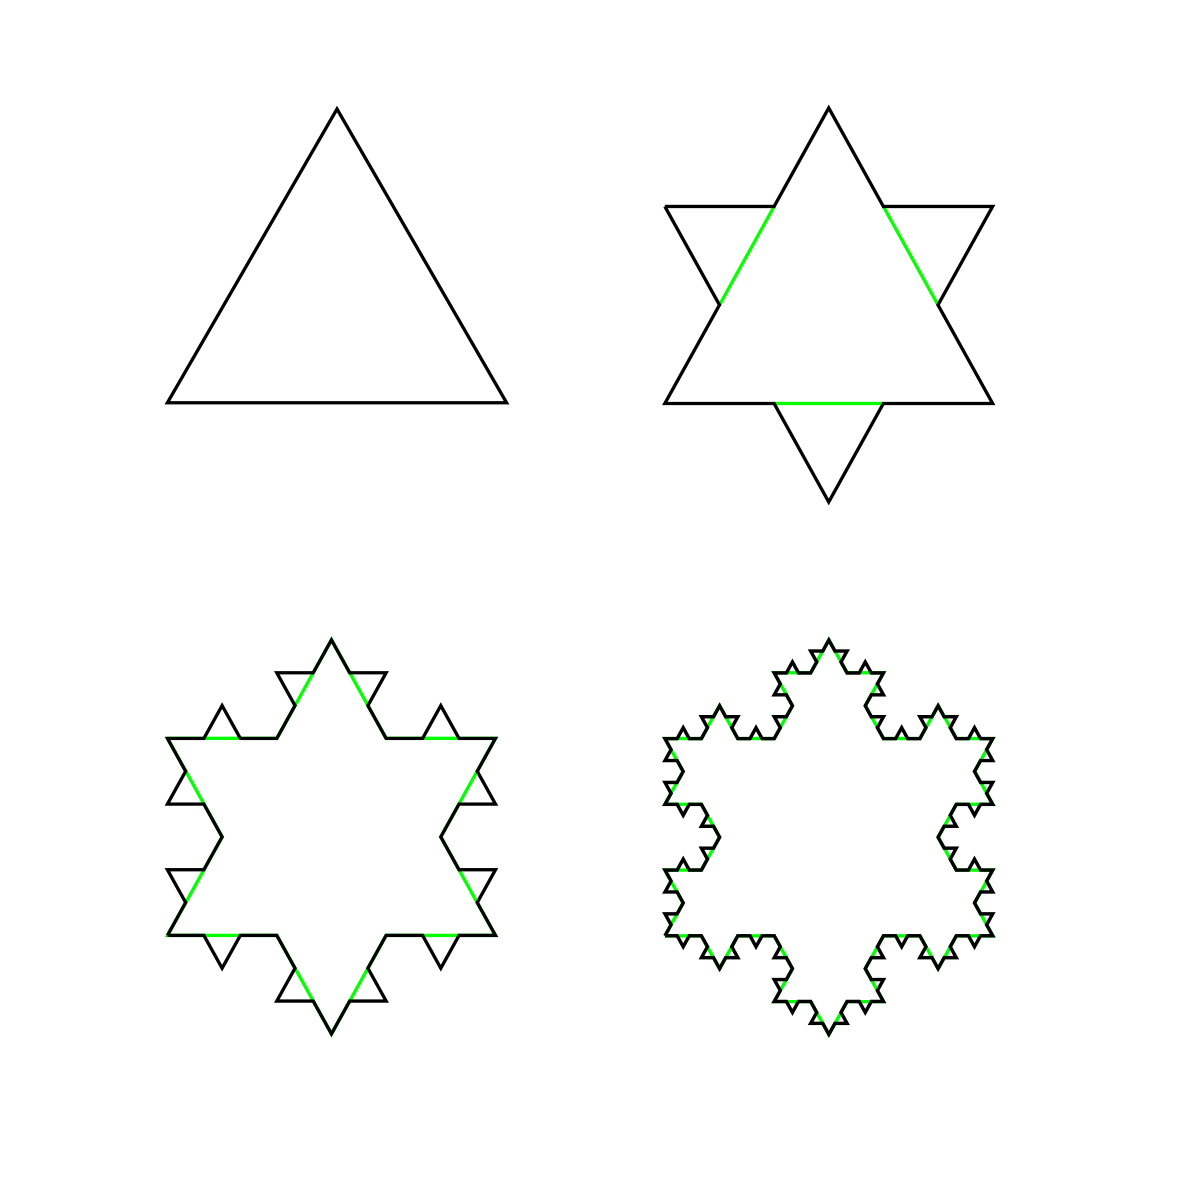
\includegraphics[width=5cm]{include/snowflake.png}
\end{center}
El copo de nieve de Koch es un poligono definido recursivamente.
Dado un poligono (un triangulo por ejemplo), se puede generar el
siguiente poligono asi:
\begin{enumerate}
        \item{Dividir cada linea del poligono en 3 partes exactas.}
        \item{Crear un triangulo nuevo en el espacio abarcado por la linea del medio
        \begin{itemize}
                \item{La longitud de cada linea del triangulo es la misma que la
                linea del medio.}
        \end{itemize}
        }
\end{enumerate}
Su tarea consiste en definir una funci\'on llamada $\mathtt{snowflake}\ :\ \mathbb{N}\rightarrow
\mathtt{List}\ (\mathbb{R},\mathbb{R})$. Esta funci\'on debe aceptar un numero natural indicando
la cantidad de veces que se repetira la recursion. Si el numero es 1, el resultado debe ser
un triangulo, similar al valor $\mathtt{fractal}$ que se definie en la linea 11 de ``Main.elm''.
\\\\
Si desea visualizar su fractal para verificar si funci\'ona correctamente, puede modificar la linea
36 de ``Main.elm'' colocando una llamada a su funci\'on con algun numero en vez de $\mathtt{fractal}$.
Por ejemplo: $\mathtt{poligono}\ ctx=\mathtt{dibujar}\ (\mathtt{snowflake}\ 5)\ ctx$. Debe volver a ejecutar $\mathtt{npm\ run\ build}$
y los resultados se pueden visualizar en \url{http://localhost:8000/index.html} al correr
$\mathtt{node\_modules/.bin/elm\ reactor}$
\section*{Triangulo de Sierpinski (10pts)}
\begin{center}
        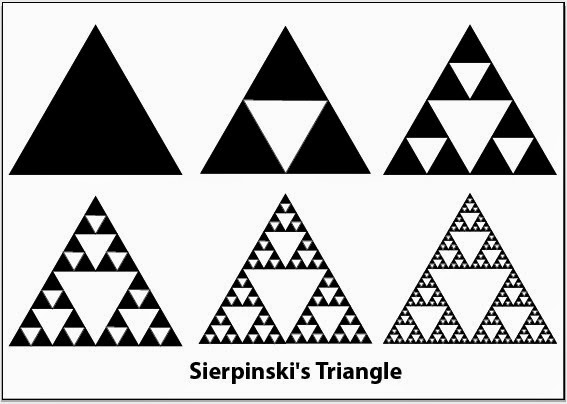
\includegraphics[width=5cm]{include/sierpinski.jpg}
\end{center}
El triangulo de Sierpinski es otro fractal generado recursivamente. El caso base consiste
en un triangulo regular. Luego, cada paso recursivo divide cada uno de los triangulos que
conforman el triangulo mediante otro triangulo que cada lado del triangulo esta ubicado en
la mitad de cada una de las lineas del triangulo anterior.
\\\\
Su tarea consiste en definir la funci\'on $\mathtt{sierpinski}\ :\ \mathbb{N}\rightarrow \mathtt{List}\ 
(\mathtt{List}\ (\mathbb{R}, \mathbb{R}))$ la cual debe aceptar un numero natural como parametro y generar
una lista de triangulos que conforman al triangulo de Sierpinski luego de aplicar la regla recursiva el
numero de veces indicado por el parametro numerico.
\\\\
Tambien debe definir la funci\'on $\mathtt{dibujarTriangulos}\ :\ \mathtt{List}\ (\mathtt{List}\ (\mathbb{R}, \mathbb{R}))
\rightarrow \mathtt{Canvas.Commands}\rightarrow\mathtt{Canvas.Commands}$. Esta funci\'on debe utilizar
la funci\'on $\mathtt{dibujar}$ que ya se definio en ``Main.elm'' en la linea 19. Para dibujar todos
los triangulos en la lista que se le ha dado. Para ello se debe:
\begin{enumerate}
        \item{Llamar la funci\'on $\mathtt{dibujar}$ con cada uno de los triangulos en la lista}
        \item{Cada llamada produce como resultado un contexto, el cual se utiliza como
        parametro para la siguiente llamada.}
        \item{Para la primera llamada, utilizar el contexto recibido como parametro}
\end{enumerate}
Meida vez hayan sido definidas estas funciones, puede dibujar su triangulo de Sierpinski modificando
la linea 45 de ``Main.elm'' con $\mathtt{poligono}\ ctx\ =\ \mathtt{dibujarTriangulos}\ 
(\mathtt{sierpinski}\ 5)\ ctx$.

\section*{Extras (15pts)}
Se otorgaran hasta 15 puntos extras por articulos adicionales en la entrega que esten relacionados
al trabajo. Algunos ejemplos podrian ser:
\begin{itemize}
        \item{Controles para decidir que fractal se debe visualizar}
        \item{Controles para controlar el numero de recursiones que
        se realizaran}
        \item{Utilizar css para mejorar la apariencia visual del programa}
        \item{Inclusion de otros fractales}
        \item{Utilizar color diferente para cada recursion dibujada para mejor
        visualizacion del fractal.}
        \item{Opcion de dibujar el fractal de forma probabilistica. Ie. a los
        puntos que conforman las esquians del fractal se les modifica la posici\'on
        ligeramente mediante numeros aleatoreos.}
        \item{Interactividad con el mouse}
\end{itemize}

\end{document}